\section{Hierarchie výpočetní složitosti. Třídy složitosti P, NP, \#P, PSPACE, EXP, NP-těžké. Definice problému Problém batohu (Knapsnack), problém směrování vozidel (VRP), Metrický k-střed.}

\subsection{Polynomická vs exponenciální časová složitost.}

Algoritmy s polynomickou složitostí lze efektivně řešit, bez vynaložení velkého výpočetního výkonu. 
S délkou vstupu \textit{n} roste lineárně potřebný čas ($n^x$) například hledání nejkratší cesty. 
Algoritmy s exponenciální složitostí lze efektivně řešit pouze pro malé exponenty, bez potřeby velkého výpočetního výkonu. 
S délkou vstupu \textit{n} roste exponenciálně potřebný čas ($x^n$) například problém obchodního cestujícího.

\subsection{Hierarchie výpočetní složitosti.}

Hierarchie výpočetní složitosti slouží k charakterizaci algoritmů u kterých lze pouze nepřímo určit asymptotickou složitost. 
Využívá se třídní hierarchie. 
Třídy od nejjednodušší po nejsložitější jdou v tomto pořadí: P $\subseteq$ NP $\subseteq$ \#P $\subseteq$ PSPACE $\subseteq$ EXP $\subseteq$ NP-složité $\subseteq$ unsolvable. 
Jednoduší třída je vždy podmnožinou složitější (do složitější patří i ty jednoduší).

\subsection{Třída P}

Třída P obsahuje polynomiální problémy. 
Tyto problémy se dají vyřešit v polynomiálním čase na deterministickém Turingově stroji (TS). 
Příkladem může být nalezení nejkratší cesty, minimální kostry v grafu.

\subsection{Třída NP}

Třída NP obsahuje nedeterministické polynomiální problémy. 
Tyto problémy lze řešit v polynomiálním čase na nedeterministickém TS (doposud nesestaven).

\subsection{Třída NP-complete (NP-úplné)}

NP-úplné (NPC) je podskupina problémů třídy NP, která se zabývá rozhodovacími problémy.
Jejich řešení je nejtěžší a všechna známá řešení lze na deterministickém TS provést pouze s exponenciálním čase. 
Pro polynomiální nebylo zatím nalezeno řešení, ale zároveň nebylo dokázáno, že řešení neexistuje.

\textbf{Problém NPC}\,--\,pokud by se podařilo, převést jeden NPC problém na polynomiální čas tak to znamená, že každý NPC problém lze převést do polynomiálního. 
To by vedlo k prokázání P $=$ NP.

Bylo dokázáno, že každý algoritmus pro NPC problém lze použít k řešení jiného NPC problému.
Přibližně existuje 10\,000 známých NPC problémů.
Příkladem může být\,--\,Barvení grafů, Knapsnack (problém batohu), 3-partition problém (rozdělit množinu čísel podmnožiny o velikosti 3, které mají stejný součet)

\subsection{Třída NP-těžké}

O problému řekneme, že je NP-težký, jestliže se na něj redukuje NPC problém, ale zároveň nevíme jestli spadá do NP.
Redukce znamená že se dá převést/konvertovat.

\subsection{P vs NP}

P je podmnožina NP jelikož každý problém lze řešit v polynomiálním čase na
 nedeterministickém TS.
Existuje matematický problém P $=$ NP, který dosud nebyl potvrzen nebo vyvrácen. Takže se přesně nedá určit jestli je P $=$ NP. 
Obecně se považuje, že P $\neq$ NP.

\subsection{Třída \#P}

Třída \#P se nezabývá rozhodovacími problémy, ale řeší problém nalezení možných řešení NP problémů. 
Z toho plyne, že problémy třídy \#P musí být alespoň stejně složité jako stejný NP problém.
U této třídy se neptáme jestli existuje řešení, ale kolik řešení existuje.

\textbf{Definice:} \#P je množina všech funkcí $f(x)$, kde $f(x)$ odpovídá počtu přijatelných cest nedeterministického TS v polynomiálním čase.

\noindent V této třídě existují také problémy \#P-úplné.

\subsection{Třída PSPACE}

PSPACE je množina rozhodovacích problémů, které lze vyřešit pomocí deterministického TS v polynomiálním paměťovém prostoru.
Neboli nezáleží, jak dlouho trvá vykonání, když je využit polynomiální (rozumné) množství paměťi. 
PSPACE má úplné problémy, které jsou sestupně samo redukovatelné (downward self-reducible) a náhodně samo redukovatelné (random self-reducible).
Jsou zahrnuté v EXP.
Dle Savitchova theorému můžeme dokázat, že \textbf{P}SPACE = \textbf{NP}SPACE.

\subsection{Třída EXP}

Často označována jako EXPTIME.
Je to množina rozhodovacích problémů řešitelných na deterministickém TS v exponenciálním čase.
Časová komplexita je O($2^{p(n)}$), kde $p(n)$ je polynomická funkce $n$.

Existuje také třída EXPSPACE, která je podobná EXPTIME, jen se neřeší v exponenciálním času, ale v exponenciálním paměťovém prostoru.

U obou tříd se jedná o nezvládnutelné problémy, pro které neexistuje polynomiální algoritmus.
Jejich složitost je exponenciální (například $2^n$).

\subsection{Knapsnack problém}

Existuje osoba (zloděj), který má batoh/zavazadlo.
Zavazadlo má určitou maximální hmotnost/velikost.
Zloděj se snaží do batohu vložit co nejvíce zboží v co největší hodnotě. 
Každé toto zboží má jinou hmotnost/velikost a jinou hodnotu.
Takže zloděj hledá co nejoptimálnější zboží, které může vložit do batohu a tím mít co největší profit.

\subsection{Problém směrování vozidel (VRP)}

Existuje 1 místo (sklad), která má x vozidel.
Vozidla ze skladu musí objet všechny místa a dovést tam zboží. 
Vozidla nemusí navštívit stejný počet míst, ale množina vozidel musí navštívit všechna místa co nejoptimálněji. 
Při jednom vozidle podobné problému obchodního cestujícího (TSP), jen s rozdílem, že u TSP si vybíráme začátek, ale u VRP máme začátek přesně definován.

\subsection{Metrický k-střed}

Máme x měst a mezi těmito městy je přesně definována vzdálenost.
Můžeme ale umístit pouze n skladišť, takže skladiště bude obstarávat více měst. 
Do některých měst chceme umístit skladiště, které bude obstarávat dalších x měst.
Musíme vybrat nejvhodnější města pro postavení skladu, aby maximální vzdálenost každého města ke skladu byla co nejmenší.


\clearpage
\section{Problém obchodního cestujícího a modifikace genetických algoritmů, Genetické programování, Optimalizace hejnem, Optimalizace mravenčí kolonií, Evoluční strategie.}


\clearpage
\section{Definice grafu. Incidenční matice, matice sousednosti. Handshaking lemma. Algoritmus detekce bipartitního grafu. Silně propojené komponenty. Kosarajův algoritmus. Tarjanův algoritmus.}

Graf je matematická struktura $G = (V, E)$: uspořádaná dvojice množin vrcholů a~hran (\emph{vertices and edges}), kde hrana je určena dvěma vrcholy a~volitelně směrem nebo váhou.
Velké množství problémů postavených nad~grafy je NP-úplných.

\subsection{Maticové reprezentace}

Incidenční matice obsahuje informace o~mapování vrcholů jednotlivým hranám.
Matice má řádek pro~každý vrchol a~sloupec pro každou hranu; pokud vrchol hraně náleží, je na~pozici jednička (pro~orientované grafy může mít výchozí vrchol hodnotu $-1$).

Matice souslednosti má podobu čtvercové matice $n \times n$ (kde $n$ je počet vrcholů grafu), jejíž hodnota na~místě $a_{i,j}$ je celé číslo odpovídající počtu hran vedoucích z~vrcholu $i$ do~vrcholu $j$, prvky na~diagonále pak odpovídají počtu hran vedoucích z~vrcholu $i$ do~vrcholu $i$.

Incidenční matice
% TODO Zde by šlo obsah matice obarvit -- pro každou hranu jiná barva.
% TODO Jak se značí když je vrchol propojený sám se sebou? Stačí tam ta jednička?
$\left( \begin{matrix}
1 & 1 & 1 & 0 & 0 & 0 & 0 \\
0 & 1 & 0 & 1 & 0 & 0 & 0 \\
0 & 0 & 0 & 1 & 1 & 0 & 0 \\
0 & 0 & 0 & 0 & 1 & 1 & 1 \\
0 & 0 & 1 & 0 & 0 & 1 & 0 \\
0 & 0 & 0 & 0 & 0 & 0 & 1 \\
\end{matrix} \right)$ 
i matice souslednosti
$\left( \begin{matrix}
2 & 1 & 0 & 0 & 1 & 0 \\
1 & 0 & 1 & 0 & 1 & 0 \\
0 & 1 & 0 & 1 & 0 & 0 \\
0 & 0 & 1 & 0 & 1 & 1 \\
1 & 1 & 0 & 1 & 0 & 0 \\
0 & 0 & 0 & 1 & 0 & 0 \\
\end{matrix} \right)$
popisují vlastnosti grafu na~obrázku \ref{ilustracni-graf-matice}.

\begin{figure}[ht]
\centering
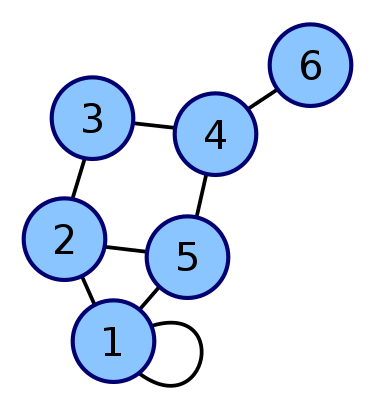
\includegraphics[height=8em]{images/3_graf-matice-souslednosti}

\caption[Ilustrační graf]{Ilustrační graf\\{\small (Chris-martin, Wikimedia Commons, volné dílo)}}
\label{ilustracni-graf-matice}
\end{figure}

\subsection{Handshaking lemma}

Handshaking lemmma je tvrzení že pro~každý konečný neorientovaný graf platí, že počet vrcholů s~lichým stupněm je sudý (formálně $\sum_{v \in V} \deg v = 2 |E|$: součet stupňů vrcholů odpovídá dvojnásobku počtu hran).

V~roce 1736 byla dokázána Leonardem Eulerem v~dokumentu řešícím problém \href{https://cs.wikipedia.org/wiki/Sedm_most%C5%AF_m%C4%9Bsta_Kr%C3%A1lovce}{Sedmi mostů města Královce}.
Graf obsahuje Eulerovskou cestu právě tehdy, když jím lze projít tak aby byla každá hrana navštívena právě jednou.

\subsection{Detekce bipartitního grafu}

Graf $G$ je bipartitní právě když je možné jeho vrcholy rozdělit do~dvou množin $V_1$ a~$V_2$ tak že každá hrana spojuje vrchol $V_1$ s~$V_2$.
Bipartitní grafy s~velikostí $|V_1|=m$ a~$|V_2|=n$ se značí $K_\mathrm{m,n}$.

Pro~detekci se využívá BFS:

\begin{enumerate}
\item Vyberte bod grafu.
\item Přiřaďte mu barvu a~označte ho za~navštívený.
\item Pokud má alespoň jeden sousední bod stejnou barvu jako aktuální bod, graf nelze obarvit dvěma barvami.
\item Všem sousedům přiřaďte druhou barvu.
\item Přejděte do~některého ze sousedů který ještě nebyl navštívený.
\item Pokračujte dokud nejsou všechny body grafu obarvené.
\end{enumerate}

\subsection{Silně propojené komponenty}

\emph{Graf} je silně propojený tehdy, když je každý vrchol dosažitelný z~každého jiného vrcholu.
Silně propojené komponenty jsou podgrafy, které jsou samy o~sobě pevně propojeny.

\subsubsection{Kosarajův algoritmus}

Algoritmus hledající silně propojené komponenty pracující v~lineárním čase.
% TODO Tato poznámka je sice pravdivá, ale není zřejmá z pseudokódu
% Využívá faktu, že transponovaný graf $G^T$ má stejné silně propojené komponenty jako původní graf $G$.

\begin{figure}[ht]
\onehalfspacing
\begin{enumerate}
\item Označ každý vrchol grafu za~nenavštívený
\item Vytvoř zásobník L
\item Pro každý vrchol grafu V spusť podprogram Navštiv(V):
    \begin{itemize}
    \item Pokud je U nenavštívený:
        \begin{enumerate}
        \item Označ U jako navštívený
        \item Pro každého souseda N zavolej Navštiv(N)
        \item Přidej U na vrchol zásobníku
        \end{enumerate}
    \item Jinak nedělej nic
    \end{itemize}
\item Pro každý vrchol V zásobníku L spusť podprogram Přiřaď(V,V):
    \begin{itemize}
    \item Pokud V nepatří žádné komponentě:
        \begin{enumerate}
        \item Přiřaď V komponentě A
        \item Pro každého souseda N zavolej Přiřaď(N,V)
        \end{enumerate}
    \item Jinak nedělej nic
    \end{itemize}
\end{enumerate}
\end{figure}
\FloatBarrier

\subsubsection{Tarjanův algoritmus}

Algoritmus hledající silně propojené komponenty pracující v~lineárním čase, efektivnější než Kosarajův.

\begin{figure}[ht]
\onehalfspacing
\begin{enumerate}
\item Označ každý vrchol grafu za~nenavštívený
\item Vytvoř zásobník
\item Vytvoř čítač \emph{i} a nastav ho na 0
\item Vyber nenavštívený vrchol \emph{v} a spusť nad ním podprogram Propoj(\emph{v}):
    \begin{enumerate}
    \item nastav \emph{v.index} a \emph{v.lowlink} na \emph{i}
    \item zvyš čítač \emph{i} o 1
    \item přidej vrchol \emph{v} do zásobníku
    \item pro každého navštívitelného souseda \emph{n}:
        \begin{itemize}
        \item pokud \emph{n} nebyl navštíven, nastav \emph{v.lowlink} na \emph{min(v.lowlink, n.lowlink)}
        \item pokud je \emph{n} v~zásobníku, nastav \emph{v.lowlink} na \emph{min(v.lowlink, n.index)}
        \end{itemize}
    \item pokud je \emph{v.lowlink} rovný \emph{v.index}:
        \begin{enumerate}
        \item vytvoř propojenou komponentu ze zásobníku
        \item vymaž zásobník
        \end{enumerate}
    \end{enumerate}
\end{enumerate}
\end{figure}
\FloatBarrier

\begin{figure}[ht]
\centering
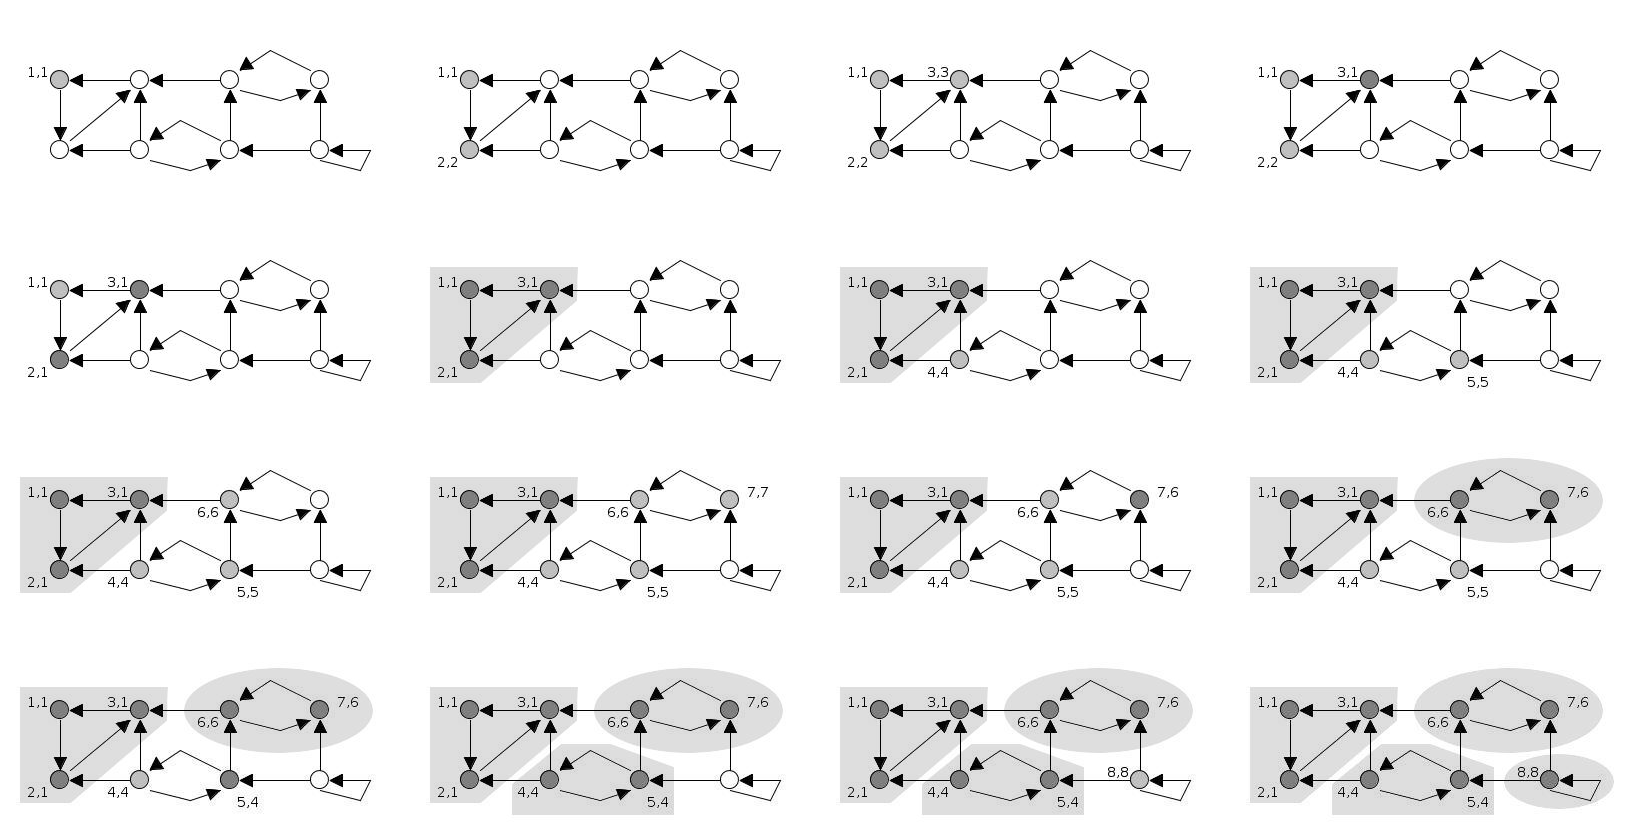
\includegraphics[width=\textwidth]{images/3_tarjanuv-algoritmus-animace.png}

\caption[Animace Tarjanova algoritmu]{Animace Tarjanova algoritmu\\{\small (LynX, Wikimedia Commons, CC BY-SA 3.0)}}
\end{figure}

\clearpage
\section{Vlastnosti grafu: průměr, excentricita. Párování grafu. Maďarský algoritmus. Problém časové tabule. Algoritmus barvení grafu. Izomorfismus grafu a Ullmanův algoritmus.}

Excentricita vrcholu $x$ grafu $G$ je maximální vzdálenost bodu od~jakéhokoliv bodu v~grafu: $\mathrm{e}(x) = \max\{ d_G(x, y) \ |\ y \in V_G\}$, kde $d_G(x,y)$ je minimální vzdálenost mezi body $x, y$.

{}Pro~poloměr grafu platí $\mathrm{r}(G) = \min\{ \mathrm{e}(x)\ |\ x \in V \}$.
\\Pro~průměr grafu platí $\mathrm{d}(G) = \max\{ \mathrm{e}(x)\ |\ x \in V \}$.

\subsection{Párování grafu}

Párování grafu je taková podmnožina hran grafu $M \subseteq E$, ve~které žádné dvě hrany nemají společný vrchol.
Vrcholy, které patří do~párování, se nazývají \emph{saturované}.

{}\emph{Maximální} párování má nejvíce hran (protože graf může mít párování více).
\\\emph{Perfektní} párování pokrývá všechny vrcholy grafu.

\subsubsection{Maďarský algoritmus}

Vstupem je matice $m \times n$ (řádky odpovídají \enquote{pracovníkům} a~sloupce \enquote{úkolům}).

\begin{enumerate}
    \item Všem polím v~každém řádku odečtěte nejnižší hodnotu řádku.
    \item Všem polím v~každém sloupci odečtěte nejnizší hodnotu sloupce.
    \item Nakreslete čáru přes řádky/sloupce tak aby překrývaly všechny nuly s~co nejmenším počtem čar (= pokrytí).
    \item Pokud je počet čar roven počtu řádků, algoritmus končí.
    \item Najděte nejmenší nepokrytou hodnotu. Odečtěte její hodnotu od~každého odkrytého řádku a~přidejte ji ke~každé nenulové hodnotě v~zakrytému sloupci. Vraťte se na krok~3.
\end{enumerate}

Výsledkem je nějaká z~kombinací nenulových polí.

\subsection{Problém časového rozvrhu}

Ve~škole je $m$ učitelů a~$n$ tříd.
Učitel $i$ musí učit v~třídě $j$ v~semestru $P_{i,j}$.
Problémem je nalezení nejlepšího řešení.

Existuje mnoho verzí tohoto problému:
limitovaný počet učeben,
učitelé mohou učit jen v~určité časy,
žáci musí mít obědovou pauzu,
v~rozvrhu by neměly být zbytečné díry,
\dots

\subsubsection{Barvení grafů}

\paragraph{Largest Degree Ordering}

Vrcholy grafu jsou seřazeny sestupně dle jejich stupně.
Prochází se jimi postupně: vrchol je obarven takovou nejdřívější barvou, která se nevyskytuje u~jeho sousedů.

\paragraph{Incidence Degree Ordering}

Je vybrán vrchol s~nejvyšším stupněm, kterému je přiřazena první barva.
Pro~neobarvené vrcholy je spočítán počet obarvených sousedů a k~obarvení je vybrán ten s~jejich největším počtem.

\subsection{Izomorfismus grafů}

Grafy $G$ a $H$ jsou izomorfní, pokud mezi nimi existuje (hrany zachovávající) bijekce (mapování).

\subsubsection{Ullmanův algoritmus}

\clearpage
\section{Problém maximálního toku a minimálního řezu grafem. Řešení problému s více zdroji a více cíly. Ford Fulkersonův algoritmus. Definice úzkého hrdla. Definice reziduální cesty.}


\clearpage
\section{Univerzální aproximační funkce. Dopředná neuronová síť. Maticová reprezentace NN. Gradientní sestup. Vrstva zahazování. Aktivační funkce. Softmax.}


\clearpage
\section{Konvoluční neuronové sítě – princip. Max pooling, Dávková normalizace. Známé architektury neuronových sítí.}


\clearpage
\section{Lineární regrese. Polynomiální regrese. Logistická regrese.}


\clearpage
\section{Rekurentní neuronové sítě. LSTM. UNet sítě. Struktury neuronových sítí.}


\clearpage
\section{Q-učení, srovnání s genetickými algoritmy.}

\clearpage
\section{Extrakce znalostí ze stromových a grafových struktur. Metoda náhodného průchodu. Node2Vec. Obecná umělá inteligence – relační induktivní zaměření, kombinatorická generalizace. Předávání zpráv.}
